\chapter{Shock Modeling}
\label{chap:3}

The focus now shifts to modeling the innovation $z_{t+1}$ in Equation~\eqref{eq:1.2}. The heterscedastic models introduced in the previous chapter help capture the excess kurtosis observed in returns. However, the distribution of the standardized return, $z_{t+1} = \frac{R_{t+1}}{\sigma_{t+1}}$, remains a challenge, as the assumption of normality is not necessarily appropriate.

Figures \ref{3.1} and \ref{3.2} display histograms of returns standardized using the conditional volatility from the GARCH(1,1) and GJR-GARCH(1,1) models, respectively. The empirical distribution of standardized returns continues to deviate from the standard normal distribution, exhibiting heavy tails, a degree of asymmetry, and a more pronounced peak around zero.\footnote{A Kolmogorov–Smirnov test performed on both sets of standardized returns strongly rejects the null hypothesis of standard normality, with p-values below 0.005\%. For an extensive survey of the approaches used in financial econometrics to assess and model non-normality in returns, see \citeA{Pagan1996}.}

\begin{figure}[H]
    \centering
    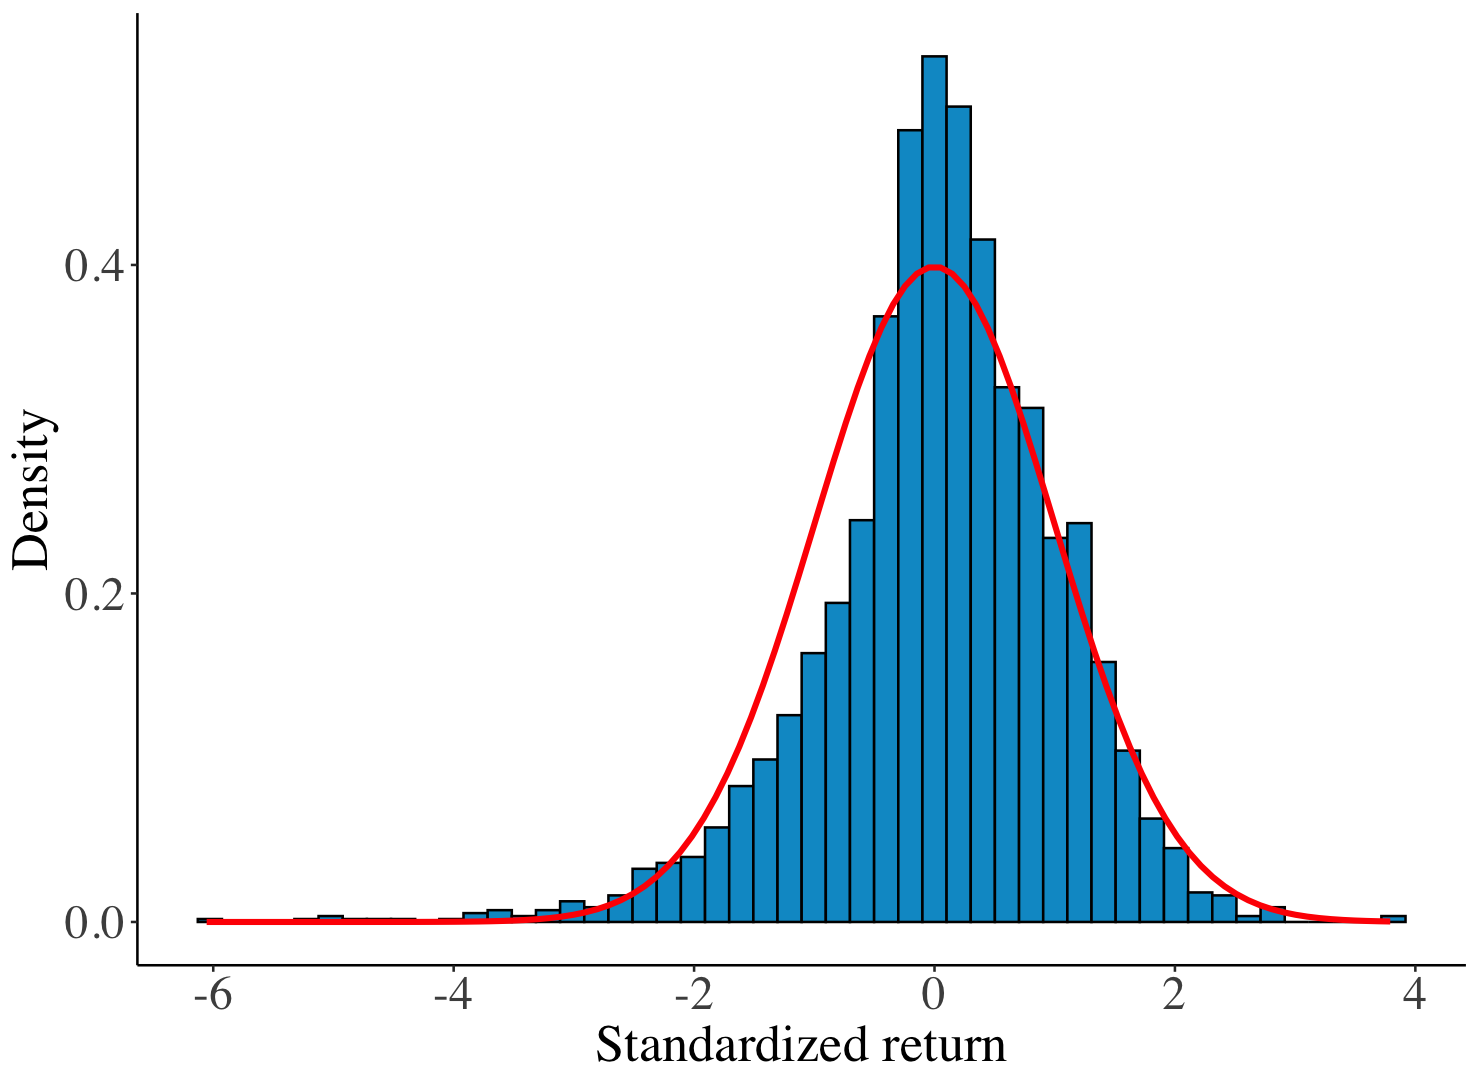
\includegraphics[scale=0.18]{../../plots/3.1.png} % Replace 
    \caption{Histogram of standardized returns, GARCH(1,1).}
    \label{3.1}
\end{figure}

\begin{figure}[H]
    \centering
    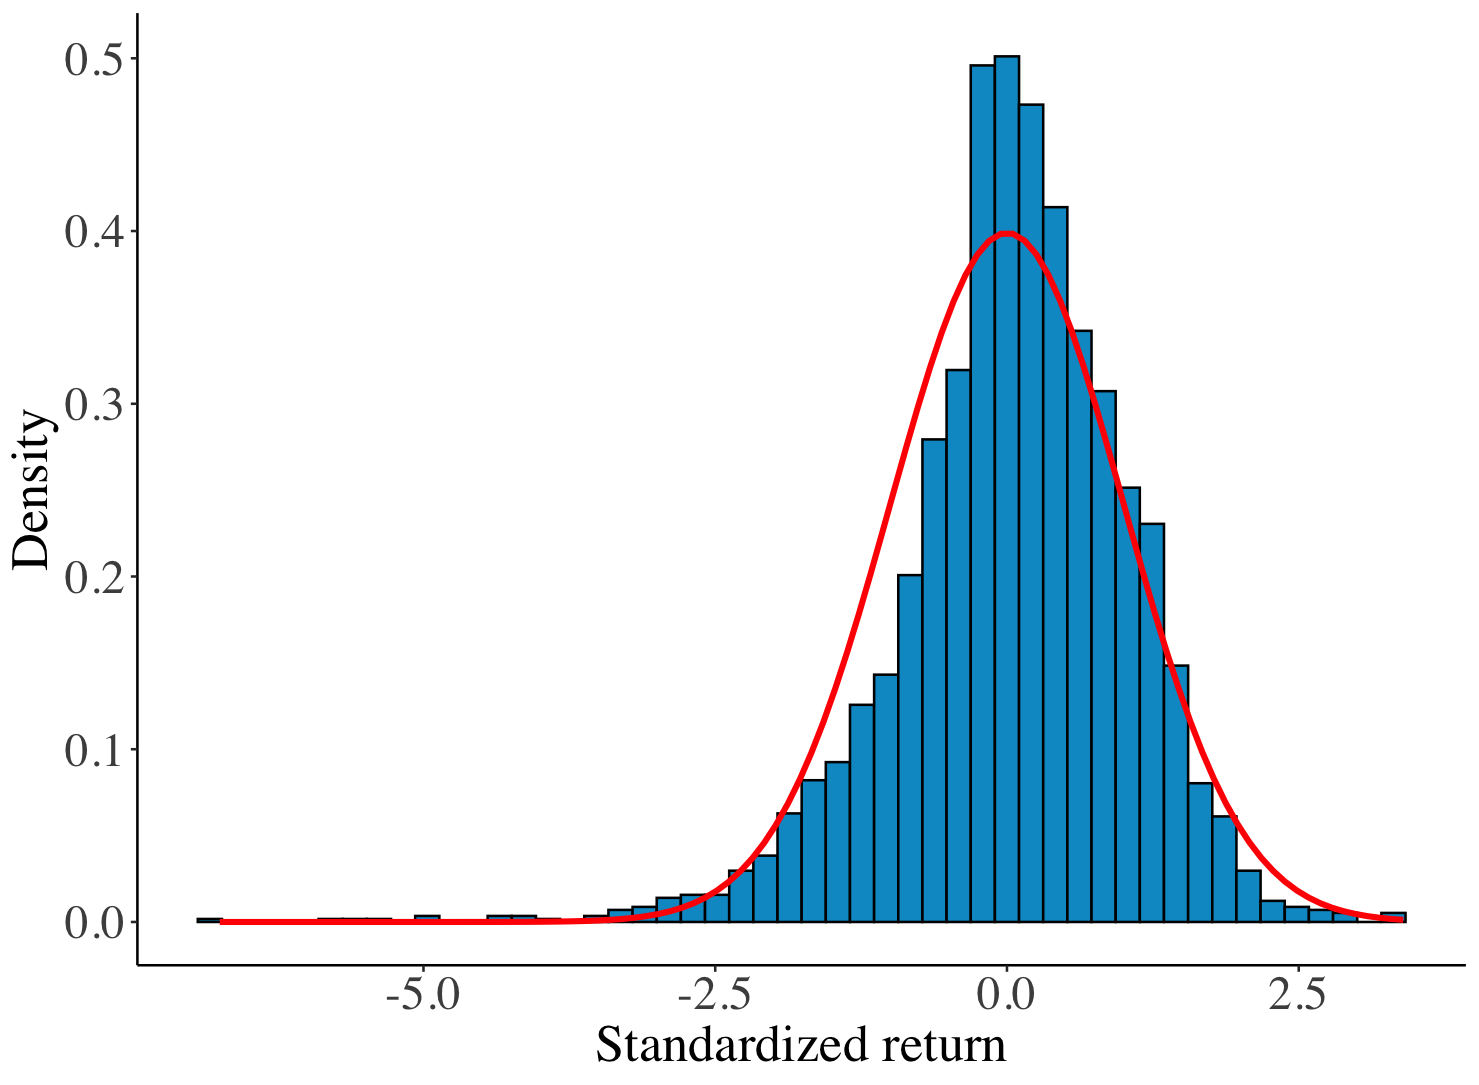
\includegraphics[scale=0.18]{../../plots/3.2.png} % Replace 
    \caption{Histogram of standardized returns, GJR-GARCH(1,1).}
    \label{3.2}
\end{figure}

\newpage

To further illustrate the limitations of the normality assumption, consider the normal QQ plots of both sets of residuals shown in Figures \ref{3.3} and \ref{3.4}. A particularly important weakness is the inability of the normal distribution to capture the left tail of the empirical distribution, which is considerably heavier. This has critical implications for risk management, as underestimating the probability of extreme negative returns leads to an underestimation of market risk.

\begin{figure}[H]
    \centering
    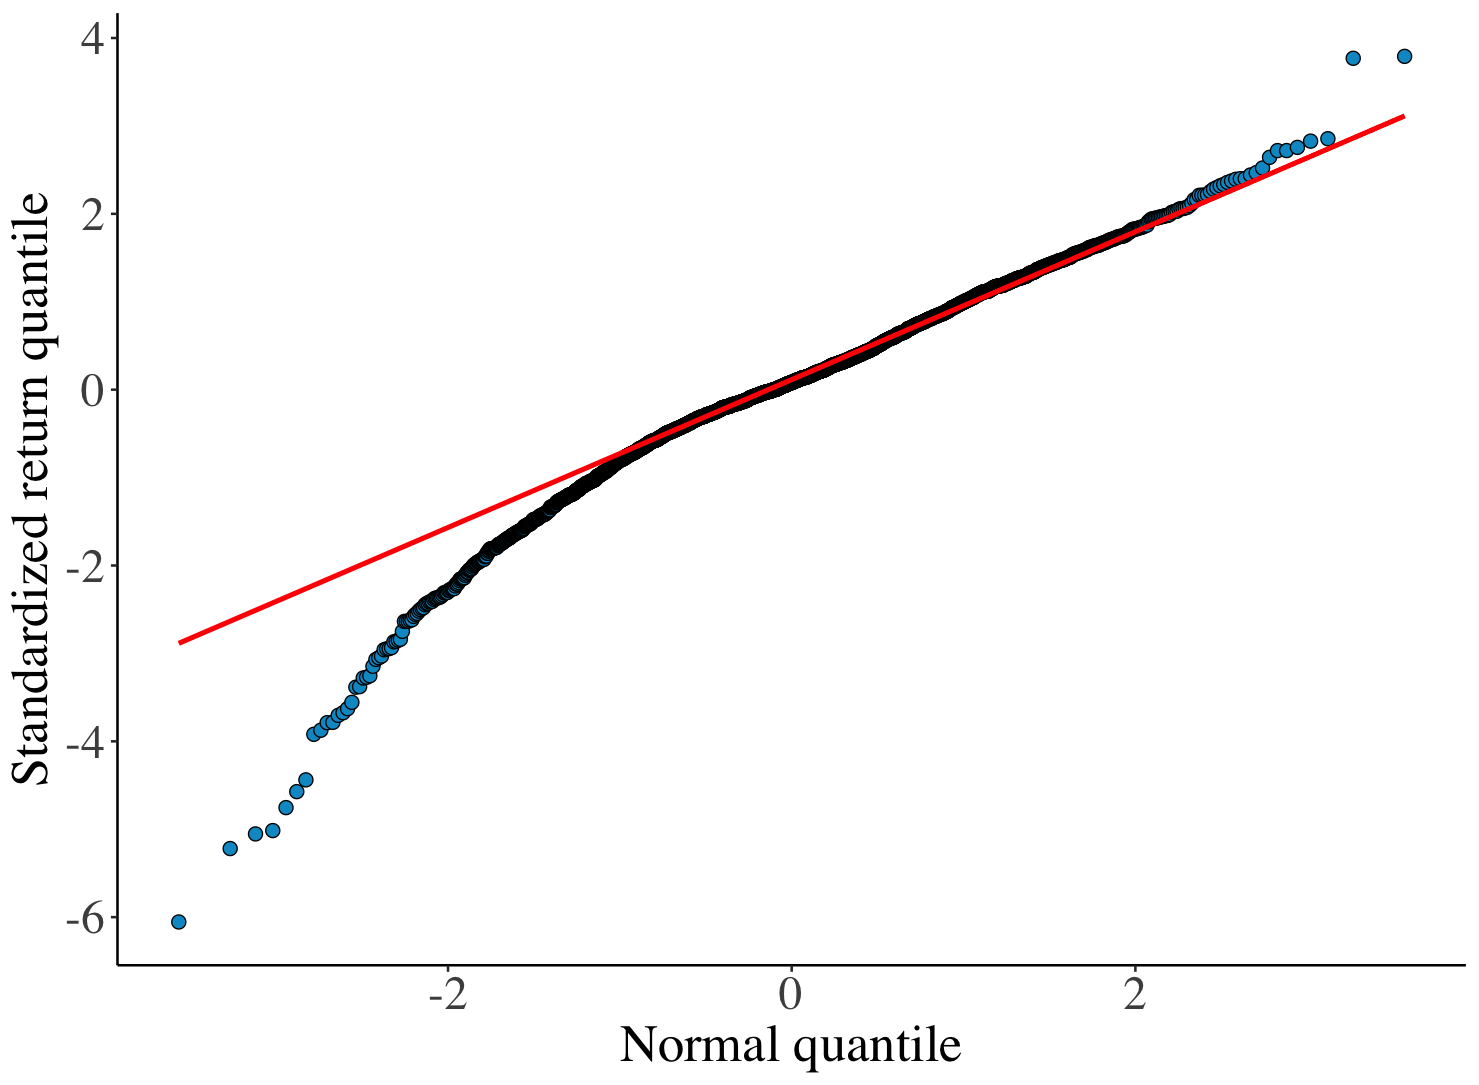
\includegraphics[scale=0.18]{../../plots/3.3.png} % Replace 
    \caption{Normal QQ plot of daily standardized S\&P 500 returns, GARCH(1,1).}
    \label{3.3}
\end{figure}

\begin{figure}[H]
    \centering
    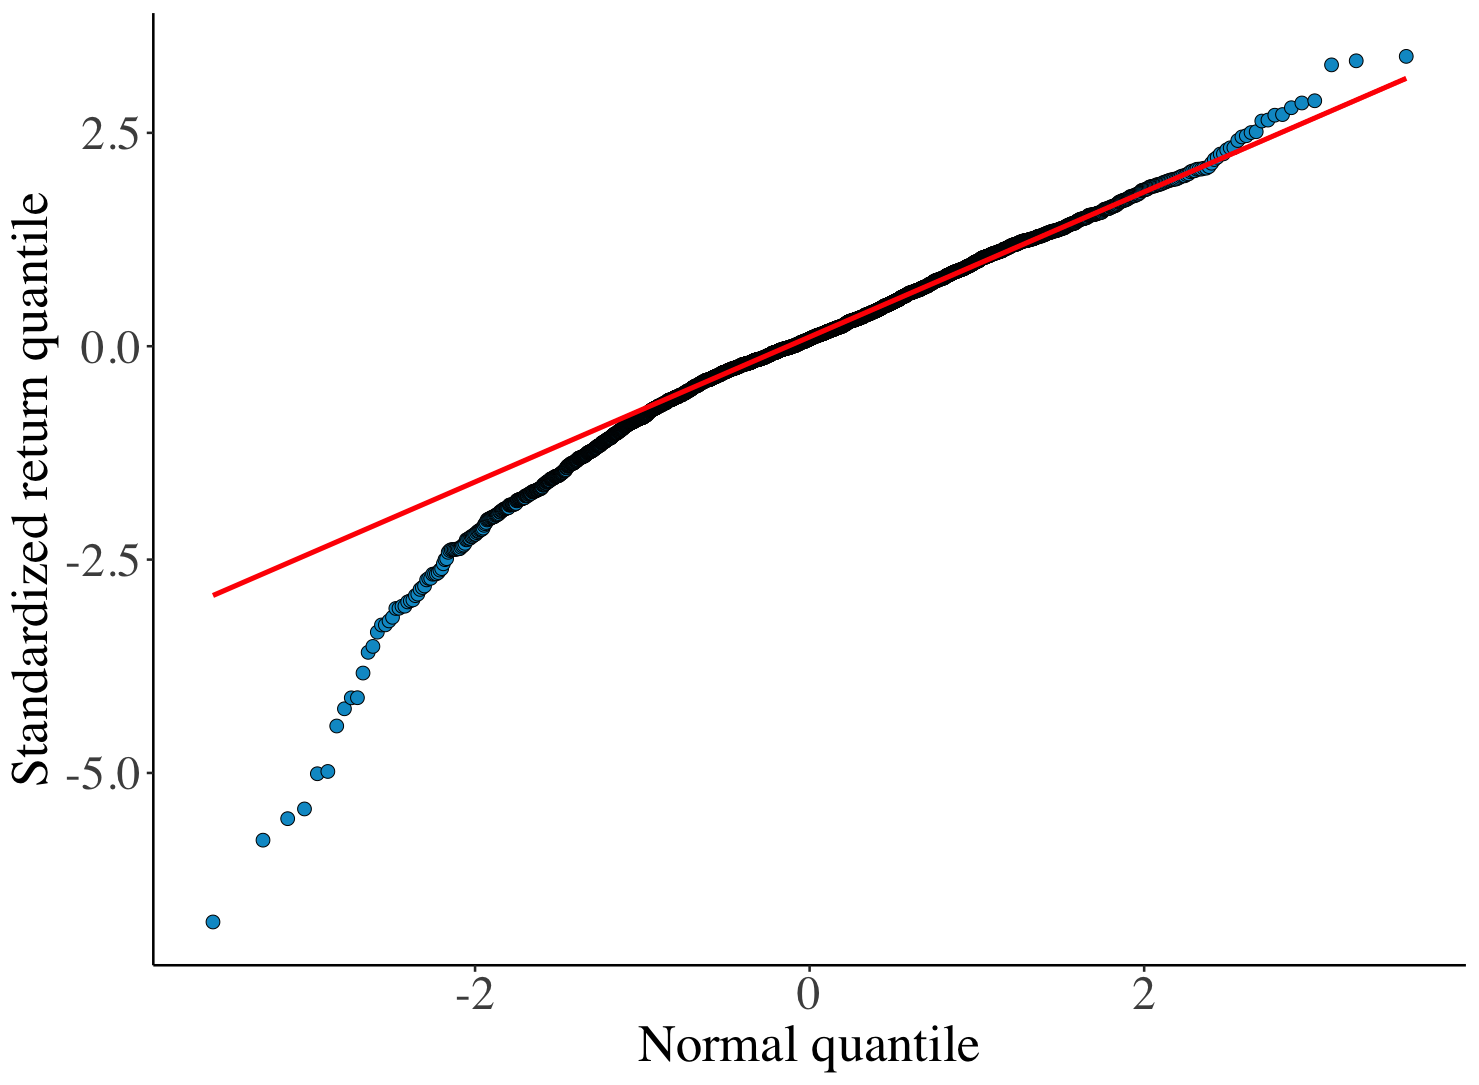
\includegraphics[scale=0.18]{../../plots/3.4.png} % Replace 
    \caption{Normal QQ plot of daily standardized S\&P 500 returns, GJR-GARCH(1,1).}
    \label{3.4}
\end{figure}
The objective is to identify a distribution that adequately fits the standardized returns, ensuring the model specified in Equation~\eqref{eq:1.2}, with the assumption $z_{t+1} \sim \text{i.i.d. } D(0,1)$, is appropriate. To overcome the limitations of the standard normal distribution, two alternative approaches are considered: an asymmetric extension of the standardized Student’s $t$-distribution, and extreme value theory.

\newpage
As \citeA{Cont2001} states, fitting various functional forms to the distribution of stock returns and stock price changes has become a popular pastime. Numerous parametric models have been proposed in the literature, starting with the normal distribution and extending to stable distributions, Student’s $t$-distribution\footnote{\citeA{Bollerslev1987} introduced an extension to the GARCH and ARCH models by allowing for conditionally $t$-distributed errors.}, and hyperbolic distributions\footnote{Stable distributions are a family of distributions closed under addition. Hyperbolic distributions are a flexible class of heavy-tailed distributions whose log-density has the shape of a hyperbola—hence the name. Because the logarithm of the density decays approximately linearly rather than quadratically in the tails, as in the normal case, hyperbolic distributions assign more probability to extreme outcomes and therefore have heavier tails than the normal distribution.}, among others. Given the empirical features discussed in \hyperref[chap:1]{Chapter 1}, a parametric distribution capable of capturing all these properties should have at least four parameters: a location parameter, a scale (volatility) parameter, a parameter governing tail behavior, and an asymmetry parameter allowing distinct behaviors for the left and right tails. The first of the approaches considered here—the asymmetric standardized $t$-distribution—meets these criteria.

The asymmetric standardized $t$-distribution, alternatively derived by \citeA{Fernandez1998}, provides a skewed extension of the Student’s $t$-distribution, enabling the modeling of both kurtosis and skewness observed in standardized returns. The probability density function (PDF) is defined as follows: 

\begin{equation}
f_{\text{asyt}}(z; d_1, d_2) =
\begin{cases}
B \thinspace C \left[ 1 + \dfrac{(Bz + A)^2}{(1 - d_2)^2 (d_1 - 2)} \right]^{-\frac{1 + d_1}{2}}, & \text{if } z < -A/B \\
B \thinspace C \left[ 1 + \dfrac{(Bz + A)^2}{(1 + d_2)^2 (d_1 - 2)} \right]^{-\frac{1 + d_1}{2}}, & \text{if } z \geq -A/B
\end{cases}
\label{eq:3.1}
\end{equation}
\noindent\text{where}
\[
A = 4\thinspace d_2\thinspace C  \thinspace  \dfrac{d_1 - 2}{d_1 - 1}, \quad
B = \sqrt{1 + 3d_2^2 - A^2}, \quad
C = \dfrac{\Gamma\left( \frac{d_1 + 1}{2} \right)}{\Gamma\left( \frac{d_1}{2} \right) \sqrt{\pi (d_1 - 2)}},
\]
and where $d_{1} > 2$, and $-1 < d_{2} < 1$. \citeA{Hansen1994} demonstrates that this is a proper density function and applies it to the U.S. Dollar/Swiss Franc exchange rate. A random variable following this distribution has zero mean, unit variance, and skewness and kurtosis that are nonlinear functions of $d_1$ and $d_2$ \cite{Christoffersen2012}. 

Thus, the first complete univariate model for daily returns is defined as:
\begin{equation}
    R_{t+1}=\sigma_{t+1}z_{t+1} \quad \text{where } z_{t+1} \sim \text{i.i.d. asyt}(d_1,d_2),
    \label{eq:3.2}
\end{equation}
with conditional variance $\sigma^2_{t+1}$ given by either the GARCH(1,1):
\begin{equation}
   \sigma^2_{t+1} = \omega + \alpha R^2_t + \beta \sigma^2_t,
    \label{eq:3.3}
\end{equation}
or the GJR-GARCH(1,1):
\begin{equation}
  \sigma^2_{t+1} = \omega + \alpha R^2_t + \alpha \theta I_t R^2_t + \beta \sigma^2_t.
    \label{eq:3.4}
\end{equation}

\citeA{Christoffersen2012} discusses various methods for estimating the model given by Equation~\eqref{eq:3.2}. In the approach followed here, the volatility parameters are first estimated using quasi-maximum likelihood estimation, and then the parameters $d_1$ and $d_2$ are estimated by maximizing the likelihood under the asymmetric Student’s $t$-distribution.

Once the parameters of the model have been estimated (the values of $d_1$ and $d_2$ for both fits are reported in Table~\ref{tab:3.1}), the goodness-of-fit can be evaluated visually and compared with the results obtained under the normality assumption. Figures~\ref{3.5} and~\ref{3.6} display histograms of standardized returns from the GARCH(1,1) and GJR-GARCH(1,1) models, respectively, along with their fitted asymmetric Student’s $t$-distributions. These figures show that the asymmetric $t$-distribution better captures both the pronounced central peak and the skewness present in standardized returns. Additionally, the tails of the fitted distribution are heavier than those of the normal distribution, offering a closer replication of the empirical characteristics.

\begin{figure}[H]
    \centering
    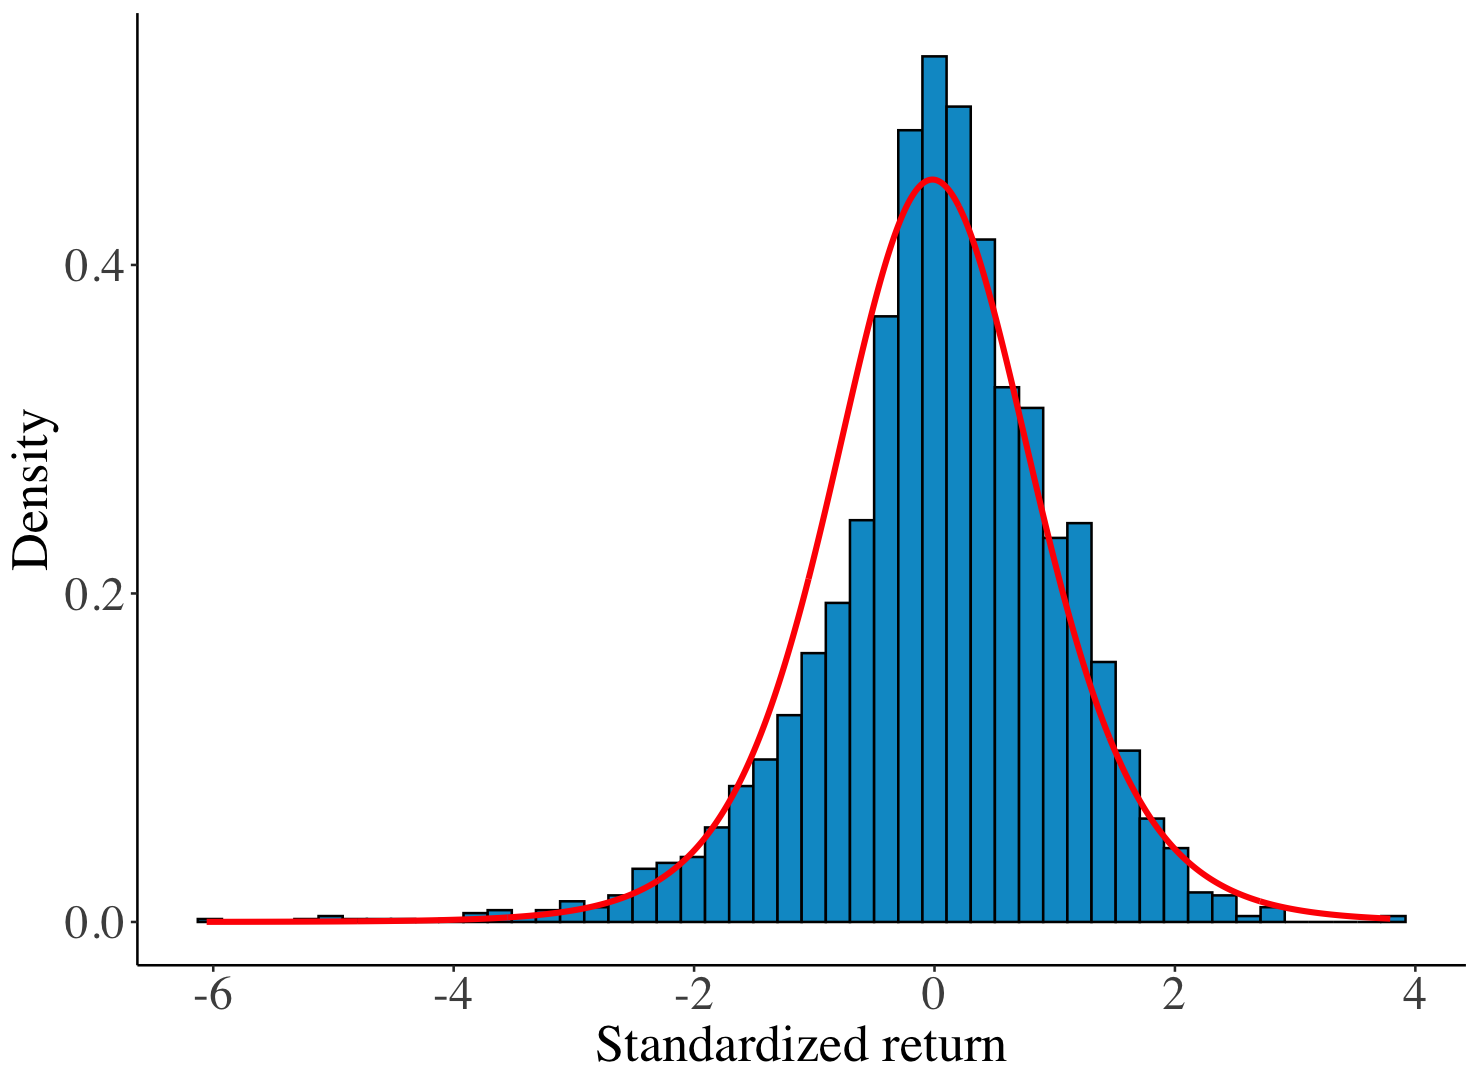
\includegraphics[scale=0.17]{../../plots/3.5.png} % Replace 
    \caption{Histogram of standardized returns with the fitted asymmetric $t$-distribution, GARCH(1,1).}
    \label{3.5}
\end{figure}

\begin{figure}[H]
    \centering
    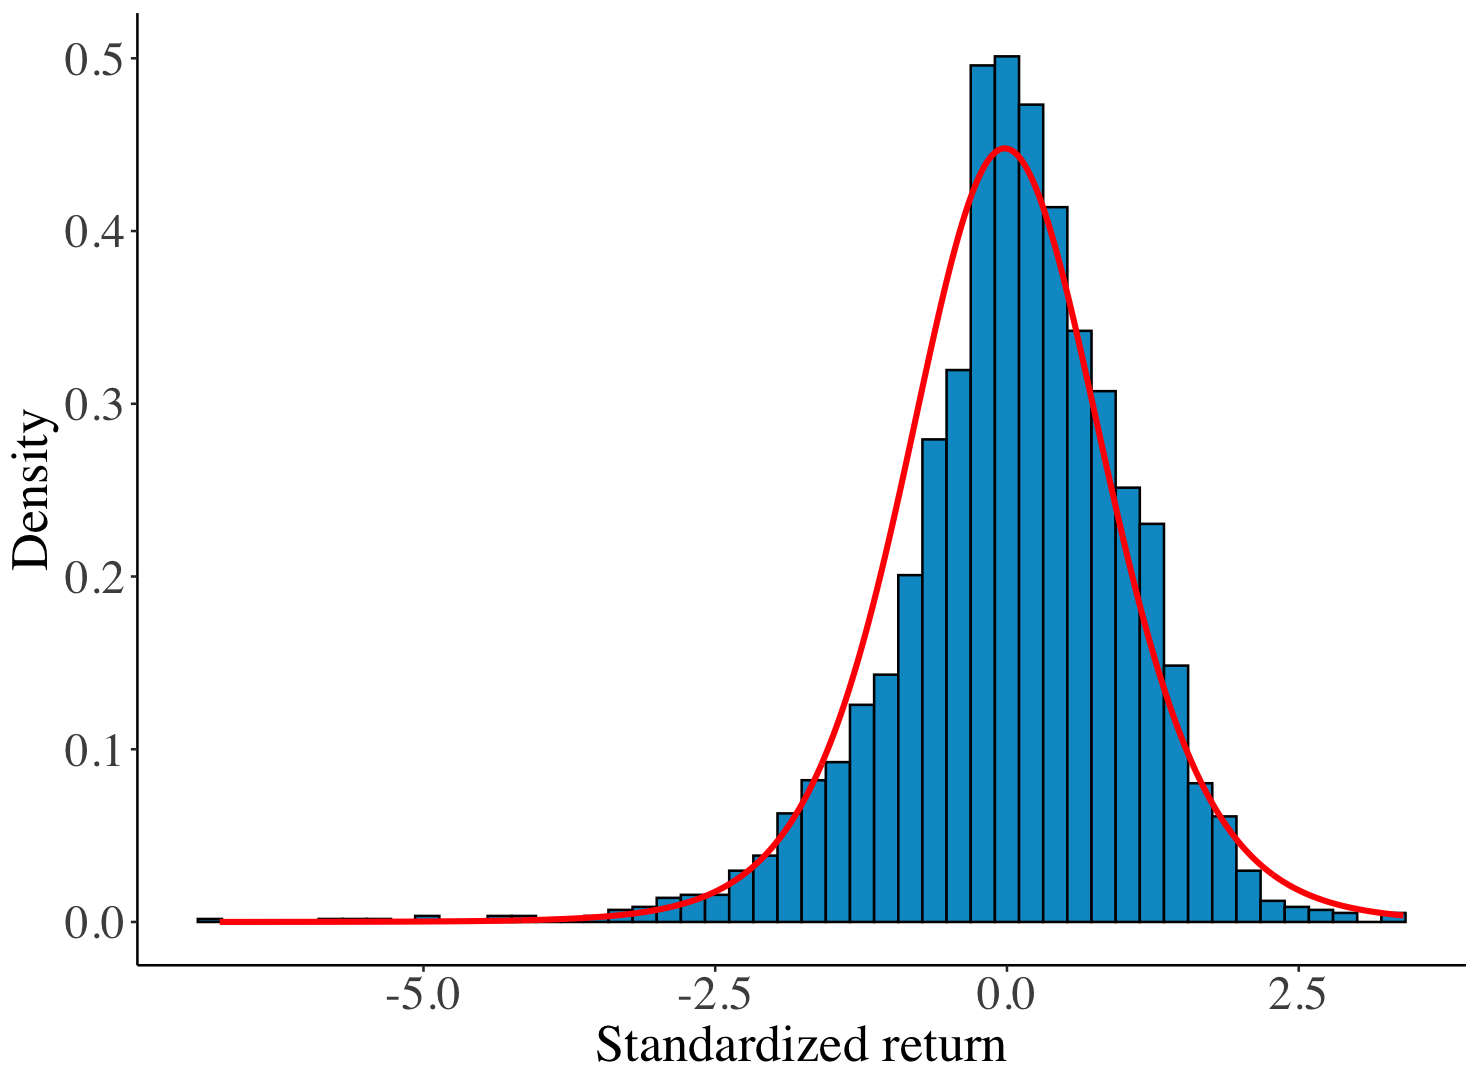
\includegraphics[scale=0.17]{../../plots/3.6.png} % Replace 
    \caption{Histogram of standardized returns with the fitted asymmetric $t$-distribution, GJR-GARCH(1,1).}
    \label{3.6}
\end{figure}

The Q–Q plots shown in Figures~\ref{3.7} and~\ref{3.8} further confirm that the asymmetric $t$-distribution provides a better fit to the standardized returns than the normal distribution. Nevertheless, the left tail of the empirical distribution remains inadequately modeled, exhibiting significantly heavier tails than those captured by the asymmetric $t$-distribution. Additionally, the comparisons between the empirical cumulative distribution functions (CDF) and their theoretical counterparts in Figures~\ref{3.9} and~\ref{3.10} reinforce the conclusion that the asymmetric $t$-distribution performs reasonably well in fitting the standardized returns.

Parametric models attempting to fit the full distribution are inevitably influenced by the high density of observations around the center, which may reduce their accuracy in capturing extreme values. For risk management, this is particularly concerning, as it risks underestimating the severity and likelihood of extreme negative returns. The inadequately modeled left tail demands special attention; thus, extreme value theory, which explicitly targets tail behavior, is introduced in the next approach. 

\begin{figure}[H]
    \centering
    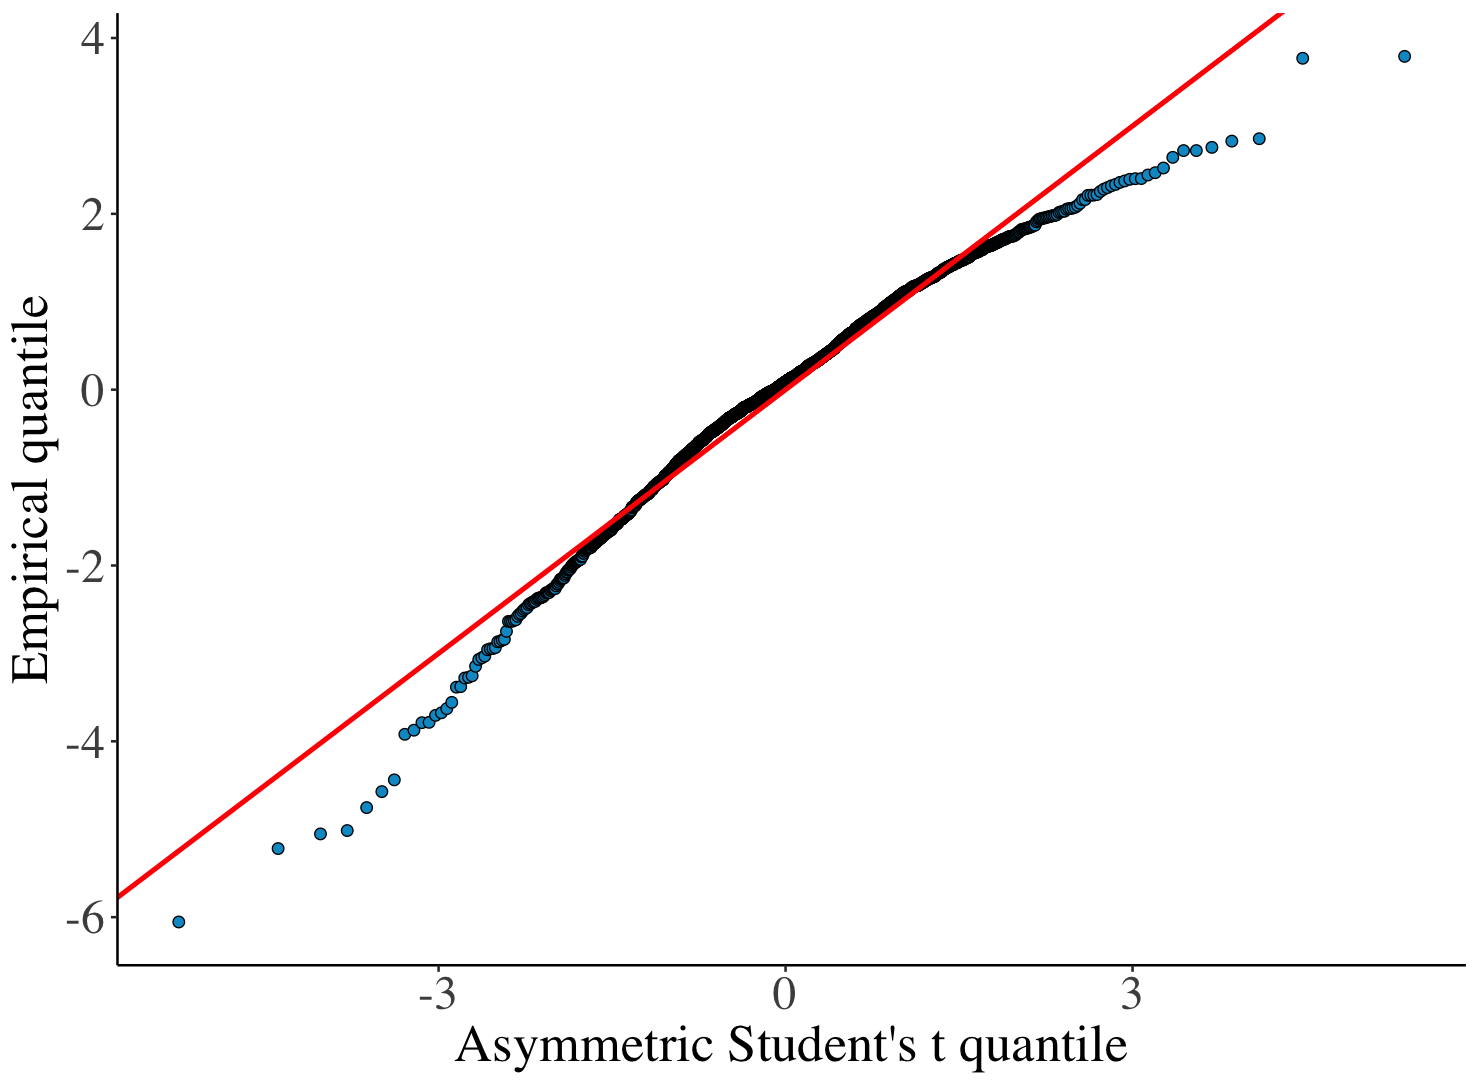
\includegraphics[scale=0.17]{../../plots/3.7.png} % Replace 
    \caption{QQ plot of standardized returns against the asymmetric $t$-distribution, GARCH(1,1).}
    \label{3.7}
\end{figure}

\begin{figure}[H]
    \centering
    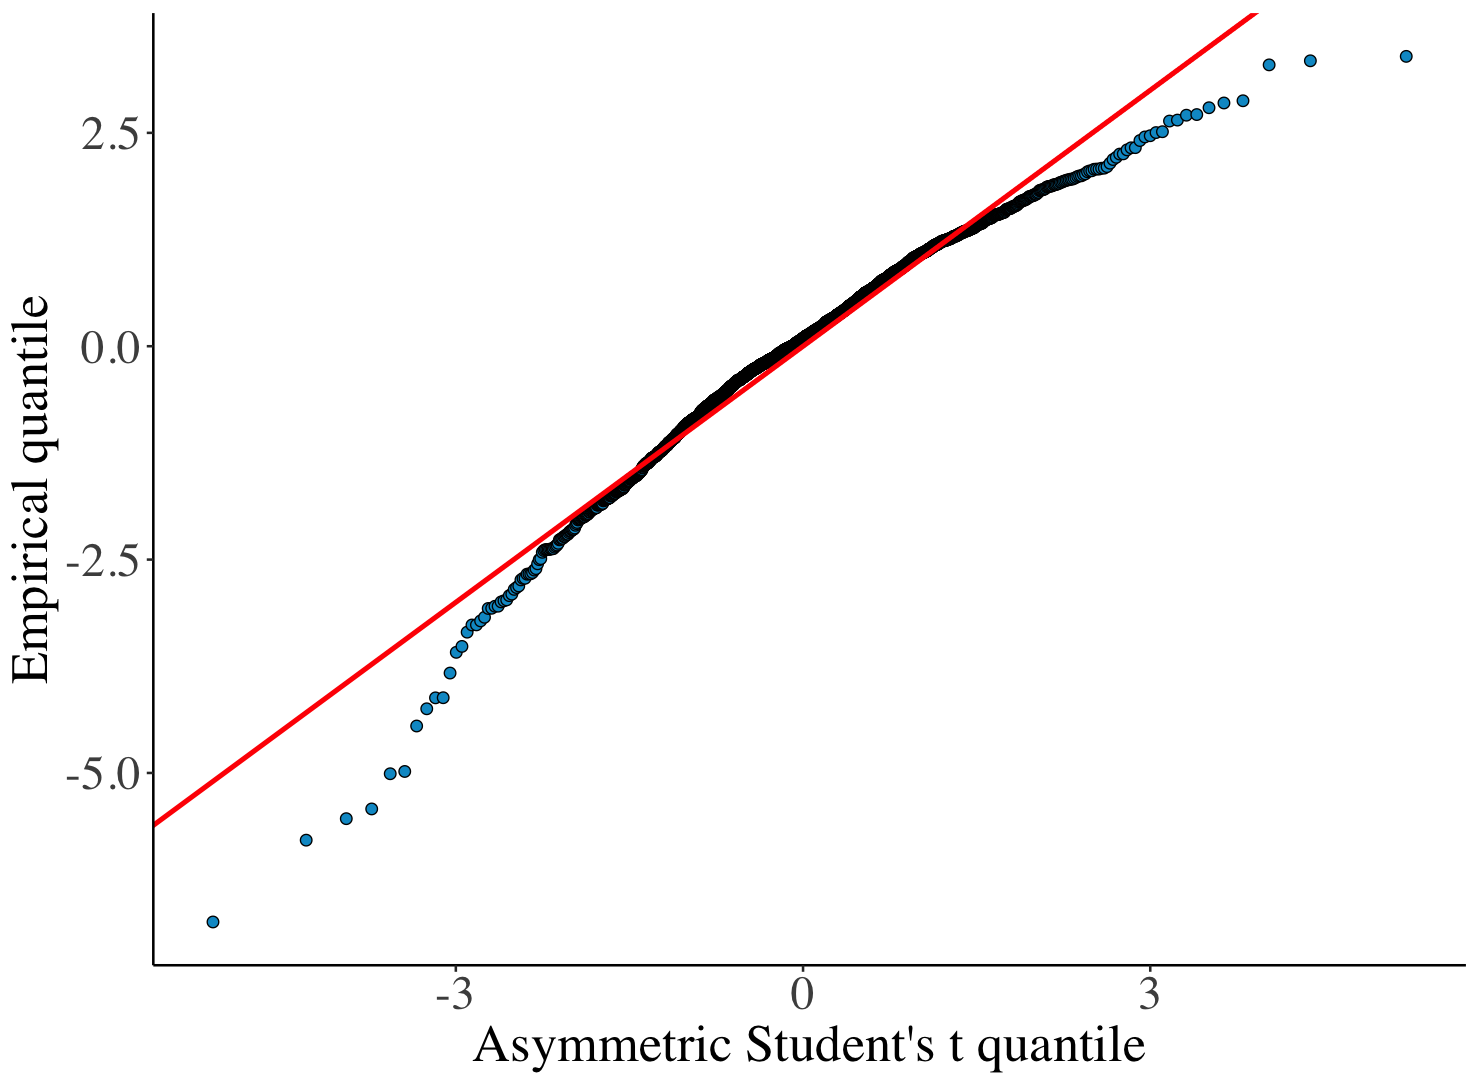
\includegraphics[scale=0.17]{../../plots/3.8.png} % Replace 
    \caption{QQ plot of standardized returns against the asymmetric $t$-distribution, GJR-GARCH(1,1).}
    \label{3.8}
\end{figure}

\begin{figure}[H]
    \centering
    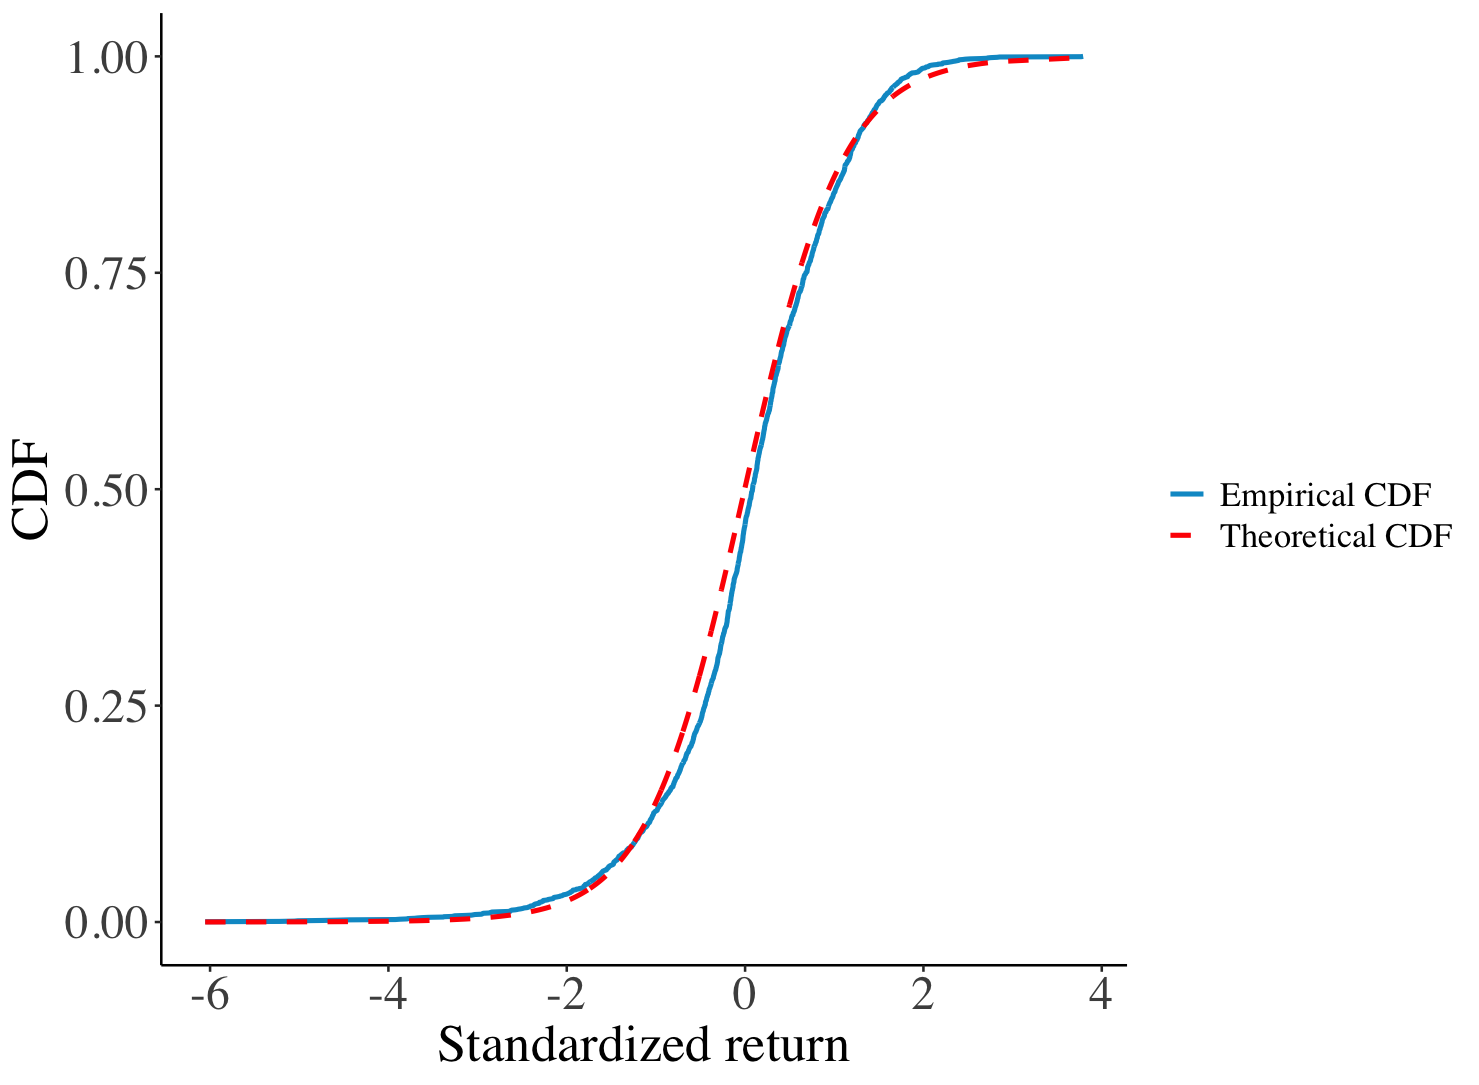
\includegraphics[scale=0.17]{../../plots/3.9.png} % Replace 
    \caption{Emprical CDF and theoretical asymmetric Student's $t$ CDF of standardized returns, GARCH(1,1).}
    \label{3.9}
\end{figure}

\begin{figure}[H]
    \centering
    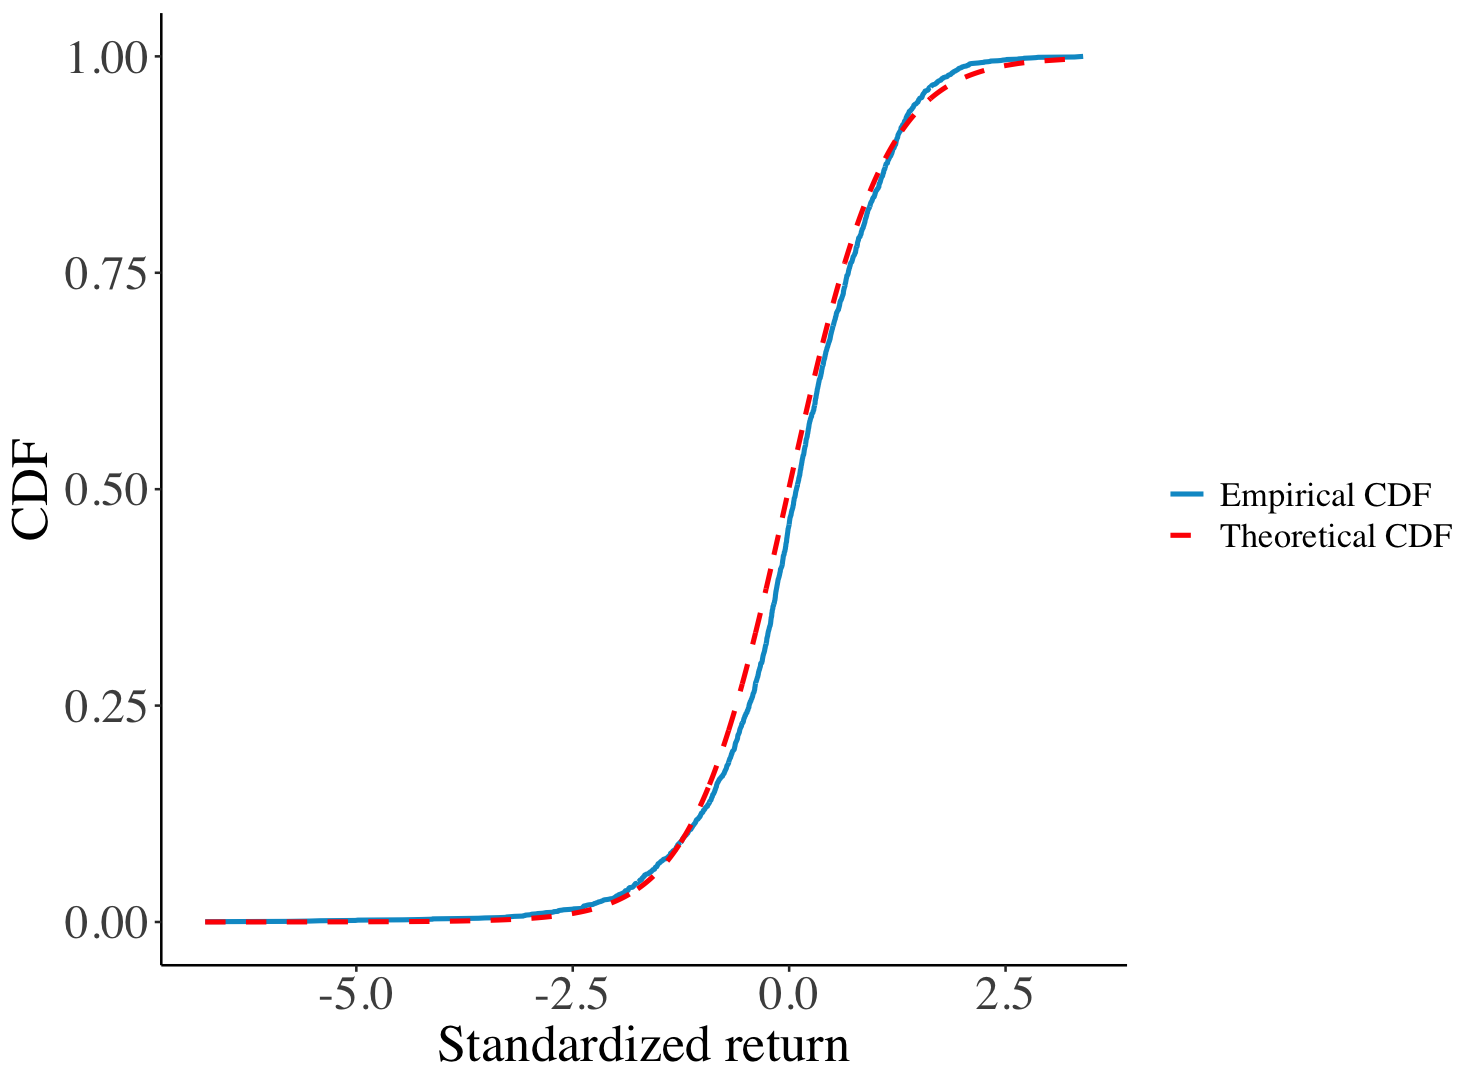
\includegraphics[scale=0.17]{../../plots/3.10.png} % Replace 
    \caption{Emprical CDF and theoretical asymmetric Student's $t$ CDF of standardized returns, GJR-GARCH(1,1).}
    \label{3.10}
\end{figure}

As noted by \citeA{Christoffersen2012}, the greatest risk to a portfolio arises from the sudden occurrence of a single large negative return. Therefore, explicit knowledge of the probabilities associated with such extreme events is central to financial risk management. Accurately modeling the left tail of the return distribution is thus critically important. Fortunately, a branch of statistics specifically addresses the modeling of these extreme events—extreme value theory (EVT).

Virtually all results in extreme value theory assume data to be independently and identically distributed (i.i.d.). Therefore, to apply this approach, the analysis is performed on standardized returns, which are assumed to meet the i.i.d. condition.

\newpage
The theoretical foundation of the approach considered here is provided by the Pickands–Balkema–de Haan theorem. This theorem states that, for a wide class of distributions $X \sim F$, given a sufficiently high threshold $u$, the conditional distribution of excesses $(X - u)$, given $X > u$, can be approximated by a generalized Pareto distribution (GPD). For a detailed statement and an outline of the proof, see \cite{Cont2001}. Consequently, the GPD naturally arises as a suitable model for the conditional tail distribution of returns, as emphasized by \citeA{Tsay2010}. Although the theorem is originally stated for the right tail, modeling the left tail simply involves applying the theorem to the negative of the returns (multiplying returns by -1).

This methodology, rooted in the Pickands–Balkema–de Haan theorem, is known in the extreme value literature as the peak-over-threshold (POT) approach. For alternative EVT-based approaches tailored specifically to financial returns, readers are referred to the chapters on extreme value theory in \citeA{Tsay2010} and \citeA{Christoffersen2012}. Further applications of EVT to financial risk management are discussed by \citeA{mcneil1999}. The particular implementation considered here was introduced by \citeA{mcneil2000estimation}.

For negative standardized returns, define $y_{t+1} = -z_{t+1}$. Then, the conditional PDF for observations exceeding a threshold $u$ is given by:
\begin{equation}
f(y; \xi, \beta, u | y>u) =
\begin{cases}
\dfrac{1}{\beta} \left(1 + \dfrac{\xi(y - u)}{\beta} \right)^{-\left(1 + \frac{1}{\xi}\right)}, & \text{for } \xi \ne 0, \; y \ge u \text{ if } \xi > 0,\; \\ & u \leq y \leq u- \frac{\sigma}{\xi} \text{ if } \xi < 0 ;\\
\\
\dfrac{1}{\beta} \exp\left(-\dfrac{y - u}{\beta}\right), & \text{for } \xi = 0,\; y \geq u.
\end{cases}
\label{eq:3.5}
\end{equation}

In the above expression, $\xi$ is the tail-index parameter, which controls the tail’s heaviness. Because financial returns exhibit tails heavier than those of the normal distribution, only the case $\xi > 0$ is considered here. In this scenario, the conditional PDF simplifies to:
\[
f(y; \xi, \beta, u | y>u) =
\dfrac{1}{\beta} \left(1 + \dfrac{\xi(y - u)}{\beta} \right)^{-\left(1 + \frac{1}{\xi}\right)}, \text{ for } \xi \ge 0, \; y \ge u.
\]

The second complete univariate model is therefore defined as:
\begin{equation}
\begin{aligned}
R_{t+1} &= \sigma_{t+1} z_{t+1}, \quad \text{where } z_{t+1} \sim \text{i.i.d. } D(0,1), \\
&\quad \quad  \quad  \quad  \quad  \quad \ \text{with } -z_{t+1} \mid (-z_{t+1} > u) \sim \text{GPD}(\xi, \beta, u),
\end{aligned}
\label{eq:3.6}
\end{equation}
and where the conditional variance $\sigma^2_{t+1}$ follows either a GARCH(1,1) or GJR-GARCH(1,1) specification.

For parameter estimation, the approach of \citeA{mcneil2000estimation} is followed. In the first step, the parameters of the volatility specification are estimated using quasi-maximum likelihood. In the second step, the parameters of the GPD are estimated via maximum likelihood using the standardized returns. \citeA{Christoffersen2012} discusses alternative estimation methods, including a semiparametric approach that is popular in the literature: the Hill estimator for the tail index $\xi$.

Before estimating the model, a threshold $u$ must be selected. As noted by \citeA{Christoffersen2012}, the choice of $u$ involves a trade-off between bias and variance: a high threshold is supported by extreme value theory but may result in too few observations, increasing variance; conversely, a low threshold provides more data but may lead to overfitting and to model misspecification by fitting observations outside the tail region. Discussions on the selection of $u$ can be found in \citeA{Tsay2010} and \citeA{coles2001}. \footnote{\citeA{Christoffersen2012} also suggests selecting $u$ by identifying the point at which the tail begins to depart from normality in the QQ plot of standardized residuals, and recommends using at least 50 observations in the tail fit, based on evidence from simulation studies.}

Fortunately, a useful property of the generalized Pareto distribution can guide this choice. For any $u > u_0$, where $u_0$ is a threshold above which the GPD provides a valid approximation, the mean excess function $e(u) = \mathbb{E}[y - u \mid y > u]$ is linear in $u$. Thus, plotting the empirical mean excess function over a range of threshold values allows identification of the region where the function becomes approximately linear—indicating a suitable choice for $u$. Figures~\ref{3.11} and~\ref{3.12} suggest that choosing $u \geq 1.8$ is reasonable for both sets of standardized returns.

\begin{figure}[H]
    \centering
    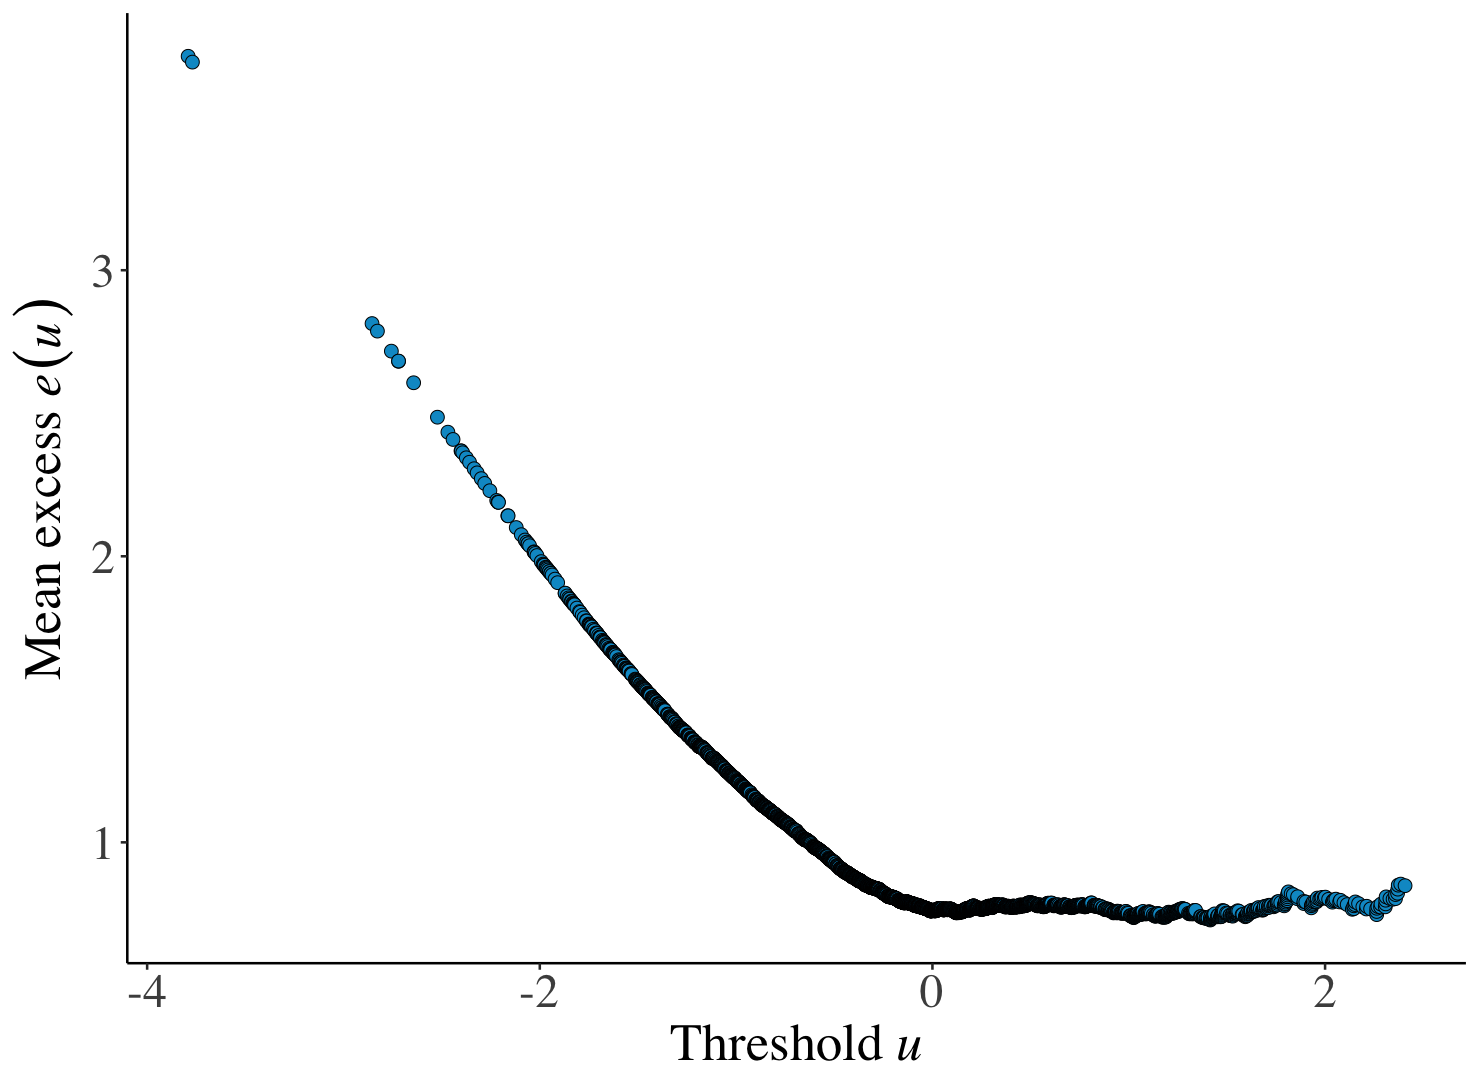
\includegraphics[scale=0.18]{../../plots/3.11.png} % Replace 
    \caption{Mean excess function $e(u)$, GARCH(1,1).}
    \label{3.11}
\end{figure}

\begin{figure}[H]
    \centering
    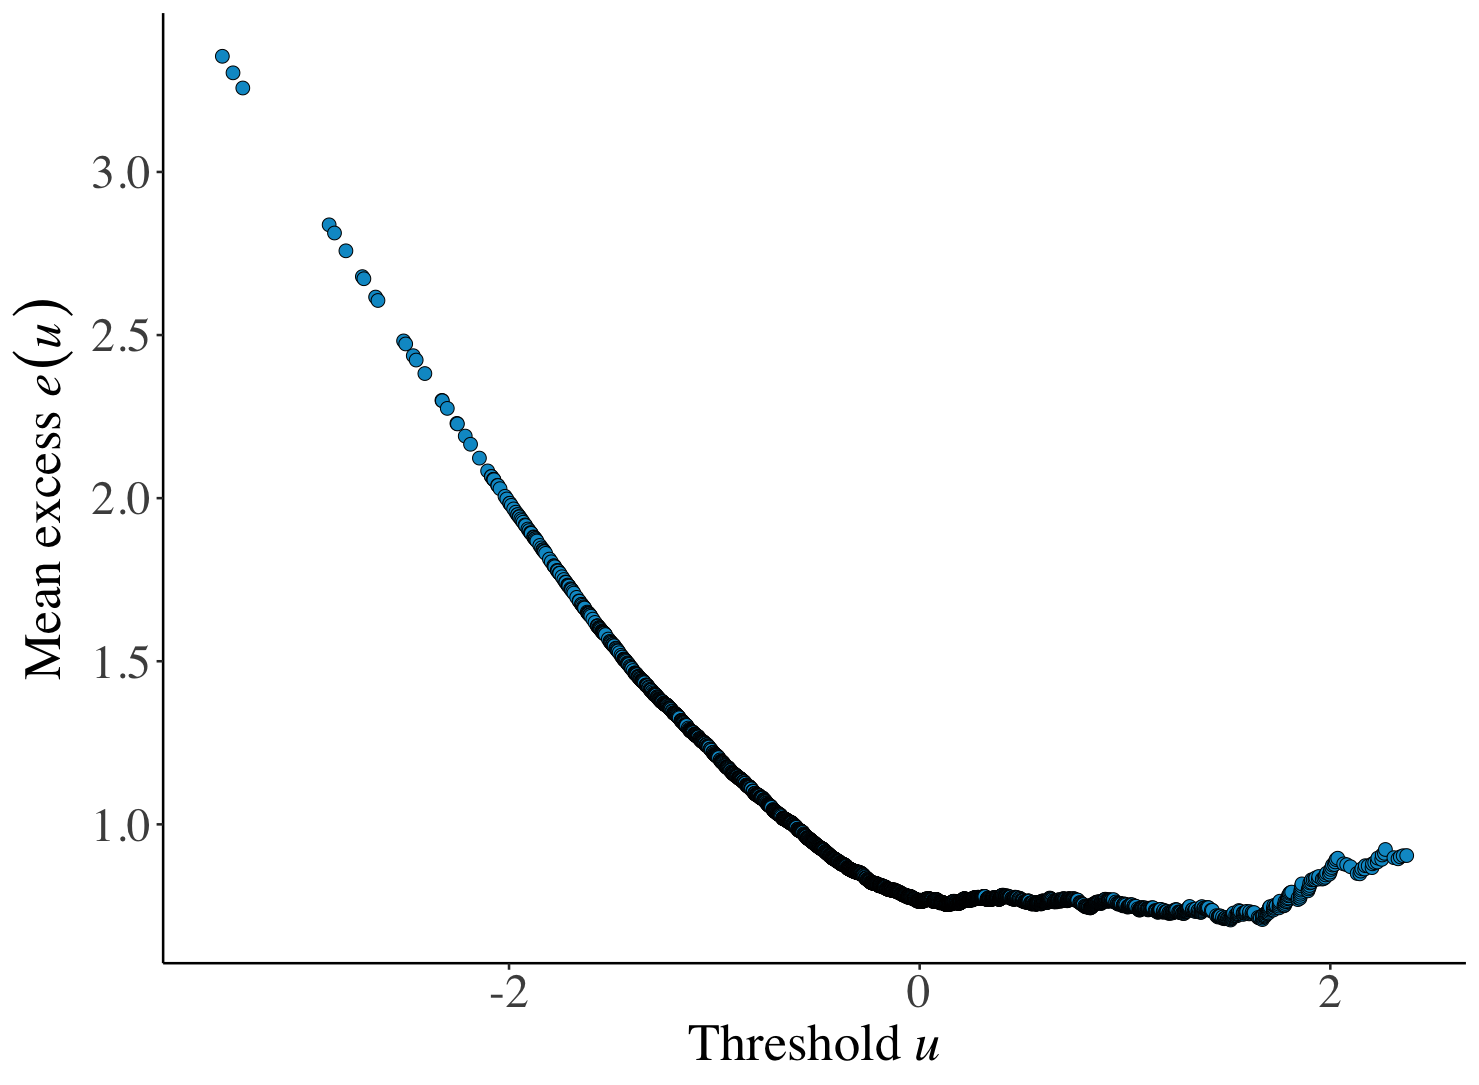
\includegraphics[scale=0.18]{../../plots/3.12.png} % Replace 
    \caption{Mean excess function $e(u)$, GJR-GARCH(1,1).}
    \label{3.12}
\end{figure}

Setting $u = 1.8$, the model in Equation~\eqref{eq:3.4} can be estimated (with the resulting GPD parameters $\beta_{\text{GPD}}$ and $\xi$ for both fits reported in Table~\ref{tab:3.1}), and the goodness-of-fit can be assessed visually. Figures~\ref{3.13} and~\ref{3.14} show that, for both sets of standardized returns—GARCH(1,1) and GJR-GARCH(1,1), respectively—the GPD provides a reasonable fit to the left tail.\footnote{The plots show the quantiles of the excesses over the threshold, along with the fitted GPD starting at zero, to aid in the visual assessment.}  However, some nuances remain, as the model’s ability to capture the tail behavior tends to diminish further into the extreme tail. To complement the visual assessment, Figures~\ref{3.15} and~\ref{3.16} display the empirical and theoretical cumulative distribution functions for both sets of standardized returns.

\begin{figure}[H]
    \centering
    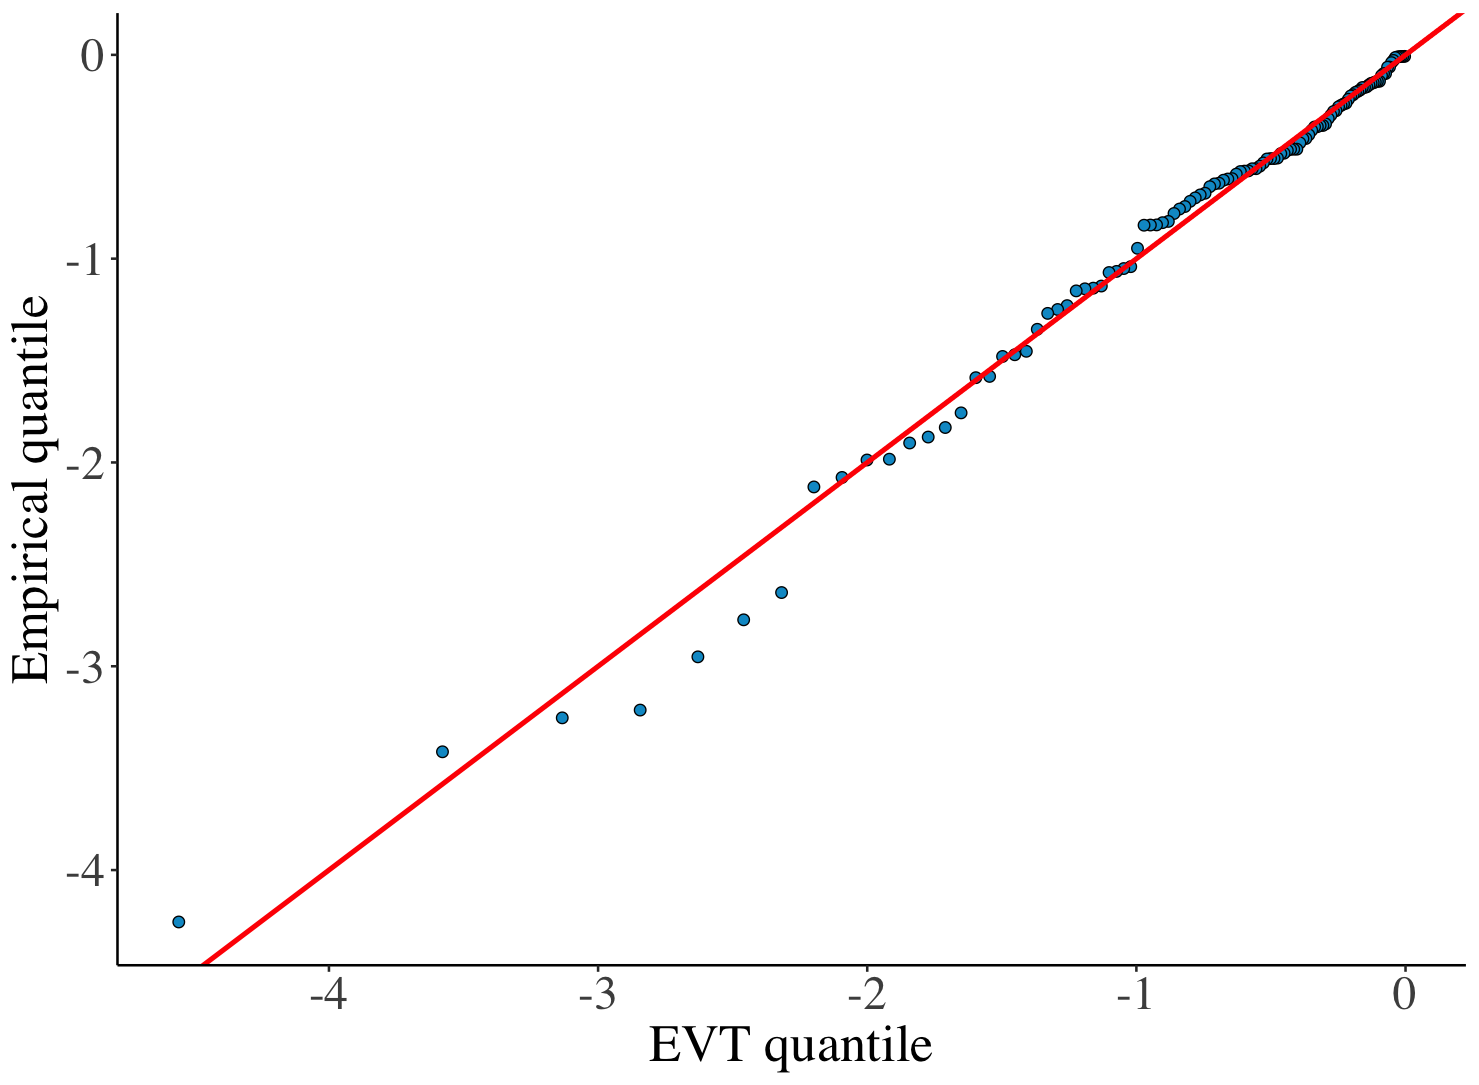
\includegraphics[scale=0.17]{../../plots/3.13.png} % Replace 
    \caption{QQ plot of standardized returns against the generalized Pareto distribution, GARCH(1,1).}
    \label{3.13}
\end{figure}

\begin{figure}[H]
    \centering
    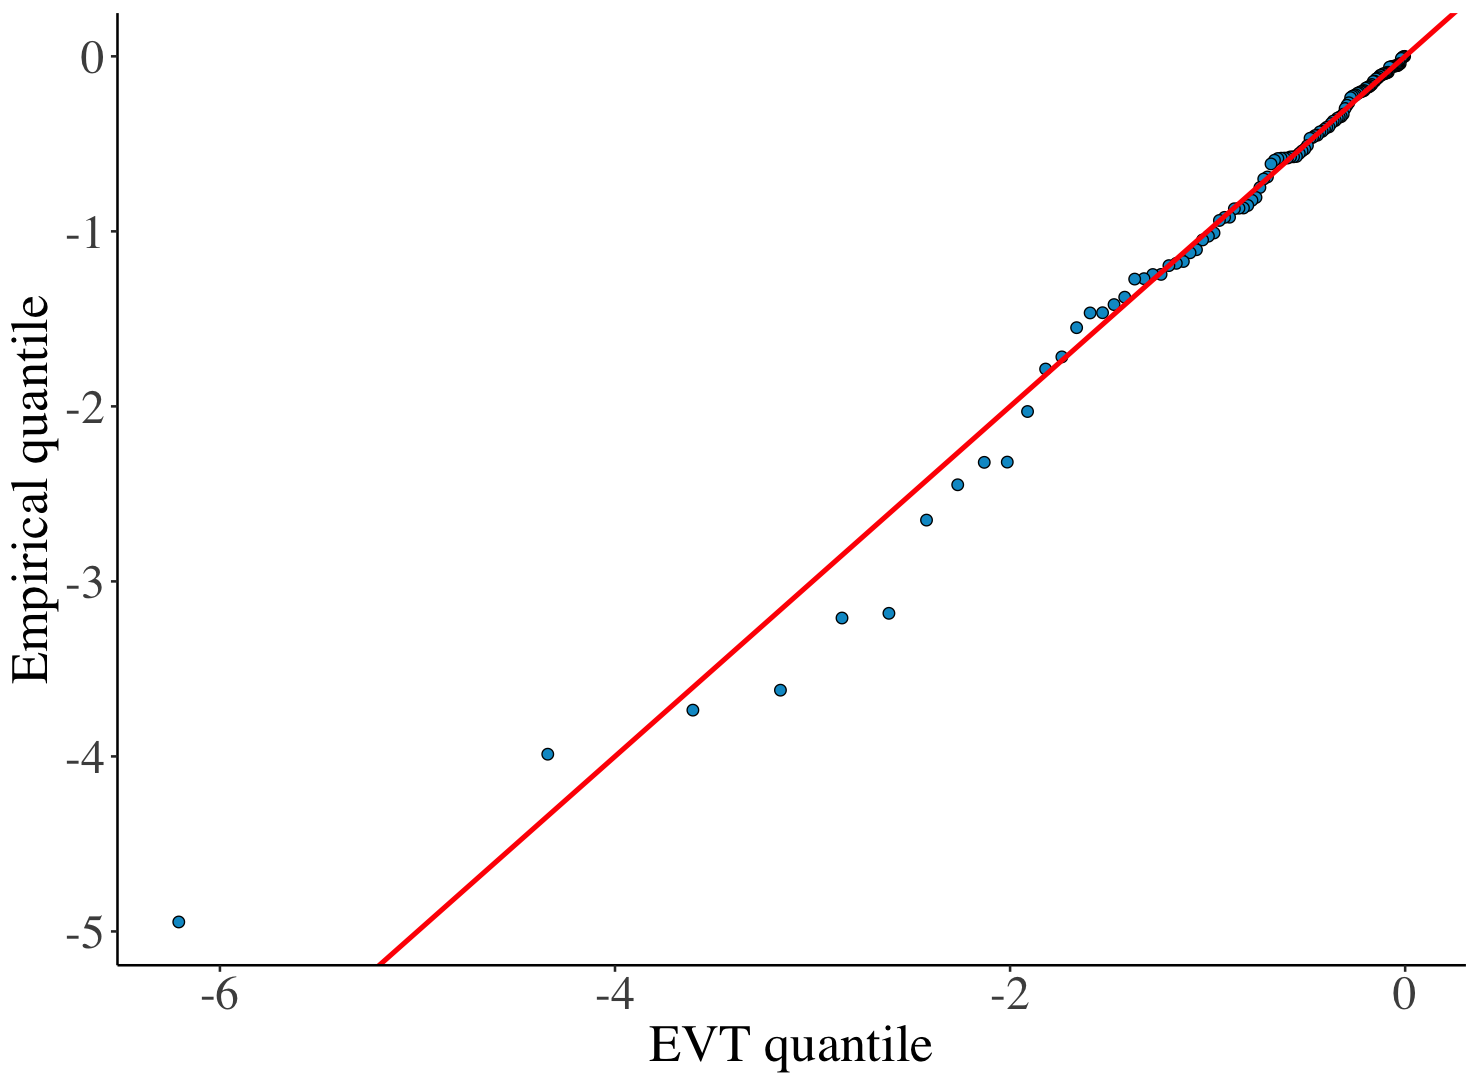
\includegraphics[scale=0.17]{../../plots/3.14.png} % Replace 
    \caption{QQ plot of standardized returns against the generalized Pareto distribution, GJR-GARCH(1,1).}
    \label{3.14}
\end{figure}

\begin{figure}[H]
    \centering
    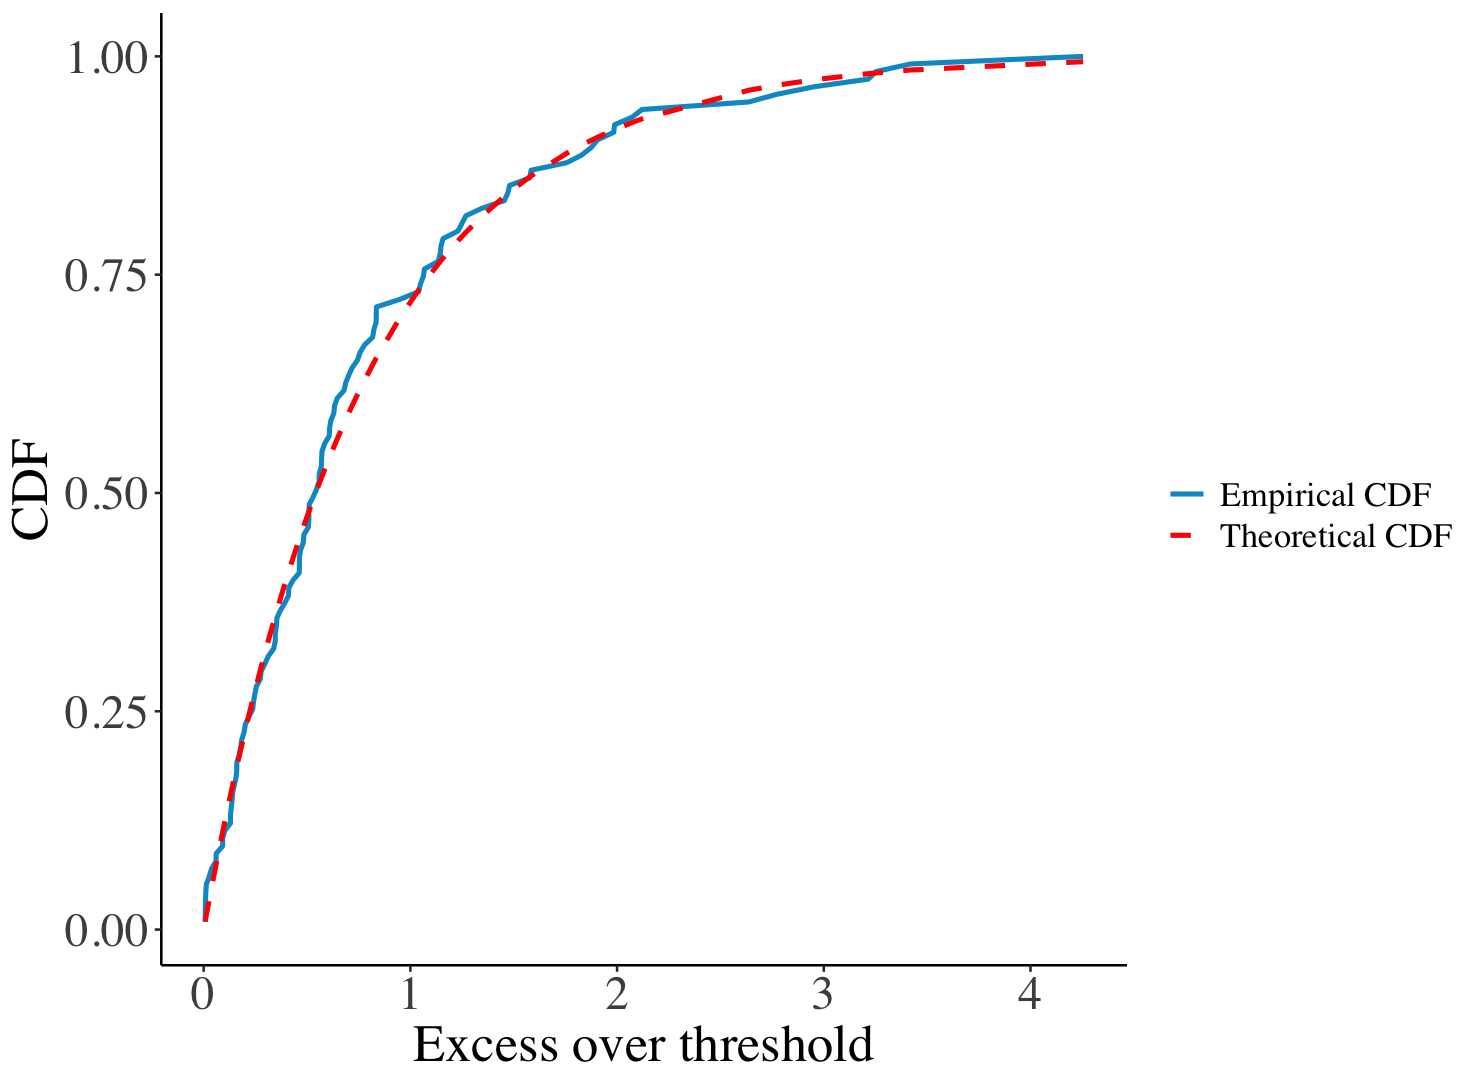
\includegraphics[scale=0.17]{../../plots/3.15.png} % Replace 
    \caption{Empirical CDF and theoretical EVT CDF of standardized returns, GARCH(1,1).}
    \label{3.15}
\end{figure}

\begin{figure}[H]
    \centering
    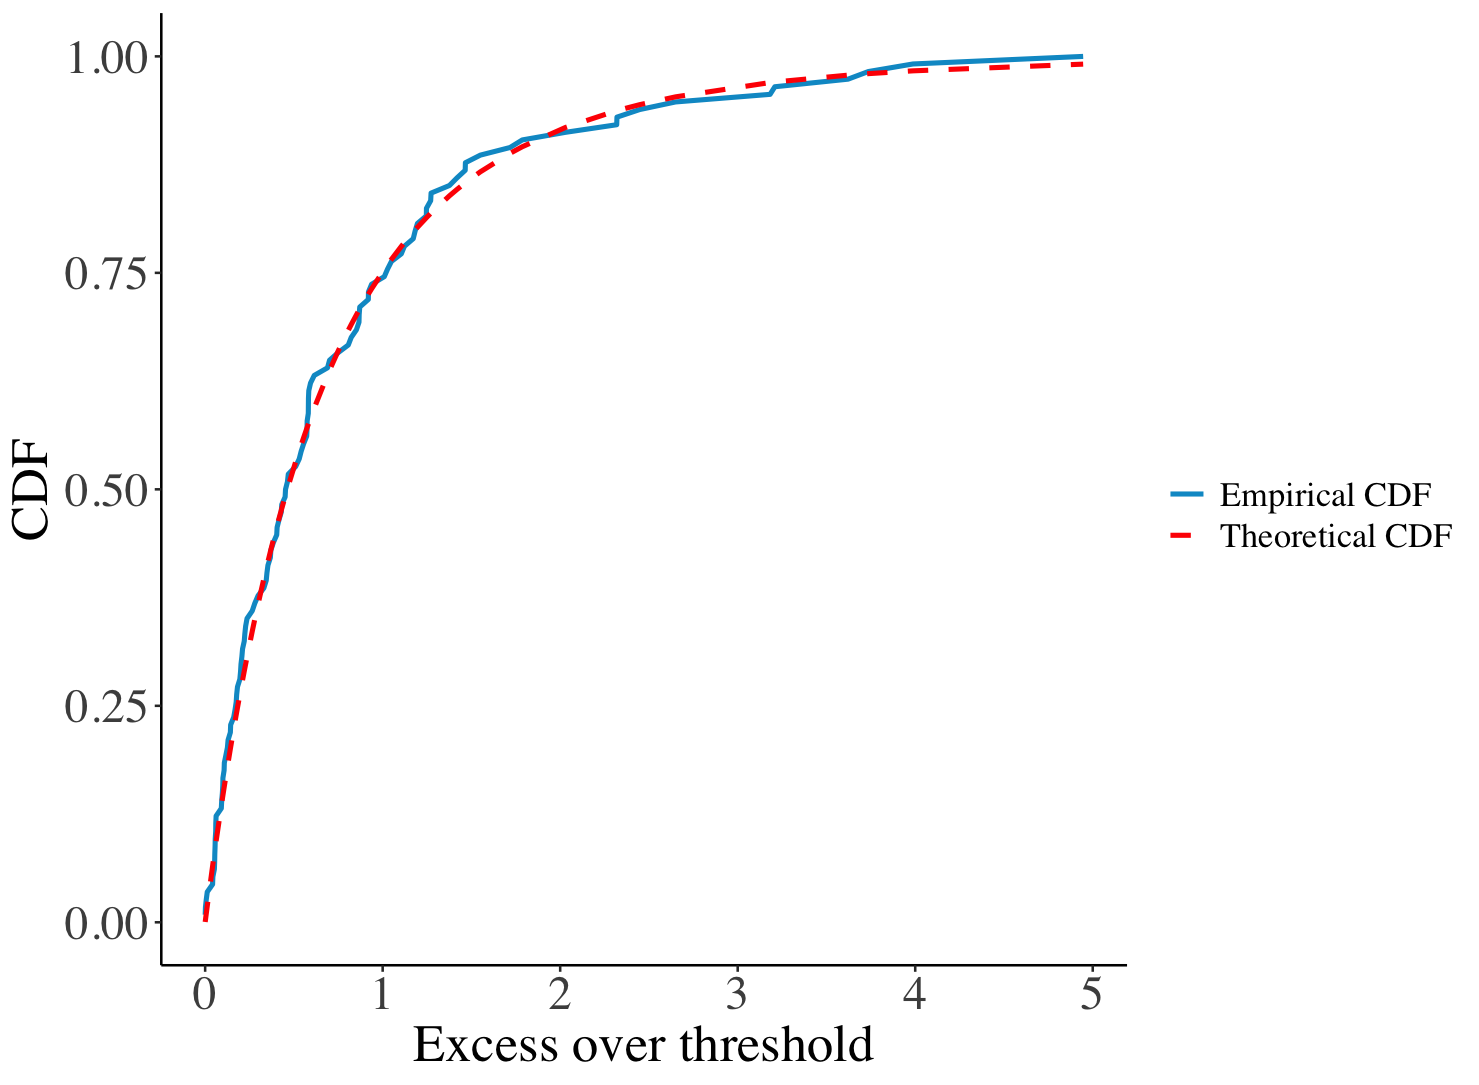
\includegraphics[scale=0.17]{../../plots/3.16.png} % Replace 
   \caption{Empirical CDF and theoretical EVT CDF of standardized returns, GJR-GARCH(1,1).}
    \label{3.16}
\end{figure}

This chapter concludes by summarizing the two approaches explored for modeling the standardized returns: the asymmetric Student’s $t$-distribution and the peak-over-threshold method derived from extreme value theory. The former is a full-distribution model aimed at capturing the entire range of return behavior, while the latter focuses exclusively on the left tail to address the shortcomings of the full-distribution approach in modeling extreme losses. In essence, the first approach provides a complete density specification, whereas the second concentrates solely on tail behavior.

The variance parameters were estimated via QMLE, after which the focus shifted to the standardized returns. In total, four models for returns were considered. Table \ref{tab:3.1} reports the estimated parameters for each model.

\begin{table}[htbp]
\footnotesize
\centering
\begin{tabular}{lcccccccc}
\toprule
\textbf{Model} & $\omega$ & $\alpha$ & $\beta$ & $\theta$ & $d_1$ & $d_2$ & $\beta_{\text{GPD}}$ & $\xi$ \\
\midrule
GARCH-Asyt &  $3.9\mathrm{e}{-6}$ & 0.171 &  0.794 & - & 7.35 & 0.0115 & - & -\\
GJR-Asyt & $4.0\mathrm{e}{-6}$ & 0.054 &  0.795 & 4.62 & 7.83 &  0.0129 & - & -\\
GARCH-EVT &  $3.9\mathrm{e}{-6}$ & 0.171 &  0.794 & - & - & - & 0.774 & 0.029 \\
GJR-EVT & $4.0\mathrm{e}{-6}$ & 0.054 &  0.795 & 4.62 & - & - & 0.621 & 0.206\\
\bottomrule
\end{tabular}
\caption{Estimated parameters.}
\label{tab:3.1}
\end{table}

In the next section, the models will be used for forecasting and evaluated from both a statistical and a risk management perspective.

\newpage